%\renewcommand{\theequation}{\theenumi}
%\begin{enumerate}[label=\thesubsection.\arabic*.,ref=\thesubsection.\theenumi]
%\numberwithin{equation}{enumi}
%
\item Show that the points 
\begin{align}
\vec{A} = \myvec{2\\-1 \\1},
\vec{B} = \myvec{1\\-3 \\-5},
\vec{C} = \myvec{3\\ -4\\-4}
\end{align}
%
are the vertices of a right angled triangle.
\\
\solution 
The following code plots Fig. \ref{fig:triangle_3d}
%
\begin{lstlisting}
codes/triangle/triangle_3d.py
\end{lstlisting}
%
\begin{figure}[!ht]
\includegraphics[width=\columnwidth]{./triangle/figs/triangle_3d.eps}
\caption{}
\label{fig:triangle_3d}
\end{figure}
%
From the figure, it appears that $\triangle ABC$ is right angled at $\vec{C}$.  Since 
\begin{align}
\brak{\vec{A}-\vec{C}}^T\brak{\vec{B}-\vec{C}}&=0
\end{align}
%
it is proved that the triangle is indeed right angled.
\item Do the points $\vec{A}=\myvec{3\\2}, \vec{B}=\myvec{-2\\-3}, \vec{C}=\myvec{2\\3} $ form a triangle?  If so, name the type of triangle formed.
\label{prob:tri_exam_coll_pts}
%
\\
\solution 

The direction vectors of $AB$ and $BC$ are 
\begin{align}
\label{eq:tri_geo_ex_baorth}
\vec{B}-\vec{A} &= \myvec{-5\\-5}
\\
\vec{C}-\vec{A} &= \myvec{-1\\1}
\label{eq:tri_geo_ex_caorth}
\end{align}
%
If $\vec{A}, \vec{B}, \vec{C}$ form a line, then, $AB$ and $AC$ should have the same direction vector. Hence, there exists a $k$ such that
\begin{align}
\vec{B}-\vec{A} &= k\brak{\vec{C}-\vec{B}}
\\
\implies \vec{B} &= \frac{k\vec{C} +\vec{A}}{k+1}
\label{eq:tri_geo_ex_caorth_section}
\end{align}
%
Since 
\begin{align}
\vec{B}-\vec{A} \ne k\brak{\vec{C}-\vec{A}},
\end{align}
%
the points are not collinear and form a triangle.  An alternative method is to create the matrix
\begin{align}
\label{eq:tri_geo_ex_diff_mat}
\vec{M} = \myvec{\vec{B}-\vec{A} & \vec{B}-\vec{A}}^T 
\end{align}
%
If $rank(\vec{M}) = 1$, the points are collinear.  The rank of a matrix is the number of nonzero rows left after doing row operations.  In this problem, 
%
\begin{align}
\vec{M} = \myvec{-5 & -5\\-1 & 1}\xleftrightarrow {R_2\leftarrow 5R_2-R_1}\myvec{-5 & -5\\0 & 10}
\\
\implies rank(\vec{M}) = 2
\end{align}
%
as the number of non zero rows is 2.
The following code plots Fig. \ref{fig:check_tri}
%
\begin{lstlisting}
codes/triangle/check_tri.py
\end{lstlisting}
%
\begin{figure}[!ht]
\includegraphics[width=\columnwidth]{./triangle/figs/check_tri.eps}
\caption{}
\label{fig:check_tri}
\end{figure}
%
From the figure, it appears that $\triangle ABC$ is right angled, with $BC$ as the hypotenuse.  From Baudhayana's theorem, this would be true if 
\begin{align}
\norm{\vec{B}-\vec{A}}^2+\norm{\vec{C}-\vec{A}}^2&=\norm{\vec{B}-\vec{C}}^2
\end{align}
which can be expressed as
\begin{multline}
\norm{\vec{A}}^2 + \norm{\vec{C}}^2 - 2\vec{A}^T\vec{C}+
\norm{\vec{A}}^2 + \norm{\vec{B}}^2 - 2\vec{A}^T\vec{B}
\\
=
\norm{\vec{B}}^2 + \norm{\vec{C}}^2 - 2\vec{B}^T\vec{C}
\end{multline}
%
to obtain 
\begin{align}
\label{eq:tri_geo_ex_orth}
\brak{\vec{B}-\vec{A}}^T\brak{\vec{C}-\vec{A}}&=0
\end{align}
%
after simplification.  From \eqref{eq:tri_geo_ex_baorth} and \eqref{eq:tri_geo_ex_caorth}, it is easy to verify that 
\begin{align}
\label{eq:tri_geo_ex_orth_sol}
\brak{\vec{B}-\vec{A}}^T\brak{\vec{C}-\vec{A}}=
 \myvec{-5 & -5}\myvec{-1\\1} = 0
\end{align}
satisfying
\eqref{eq:tri_geo_ex_orth}. Thus,  $\triangle ABC$ is right angled at $\vec{A}$.
%
%
%\item Area of a triangle is half the product of its base and the corresponding altitude. 
%%
%\\
%\solution First, we consider the right angled triangle in Fig\ref{fig:tri_right_area}. By definition, the area of the rectangle $ABCD$ is $ac$.  Also, The rectangle is a sum of two congruent triangles $ABC$ and $ADC$.  Thus,
%%
%\begin{align}
%\text{ar}\triangle ABC=\text{ar}\triangle ADC = \frac{1}{2}ac
%\end{align} 
%%
%\begin{figure}[!ht]
%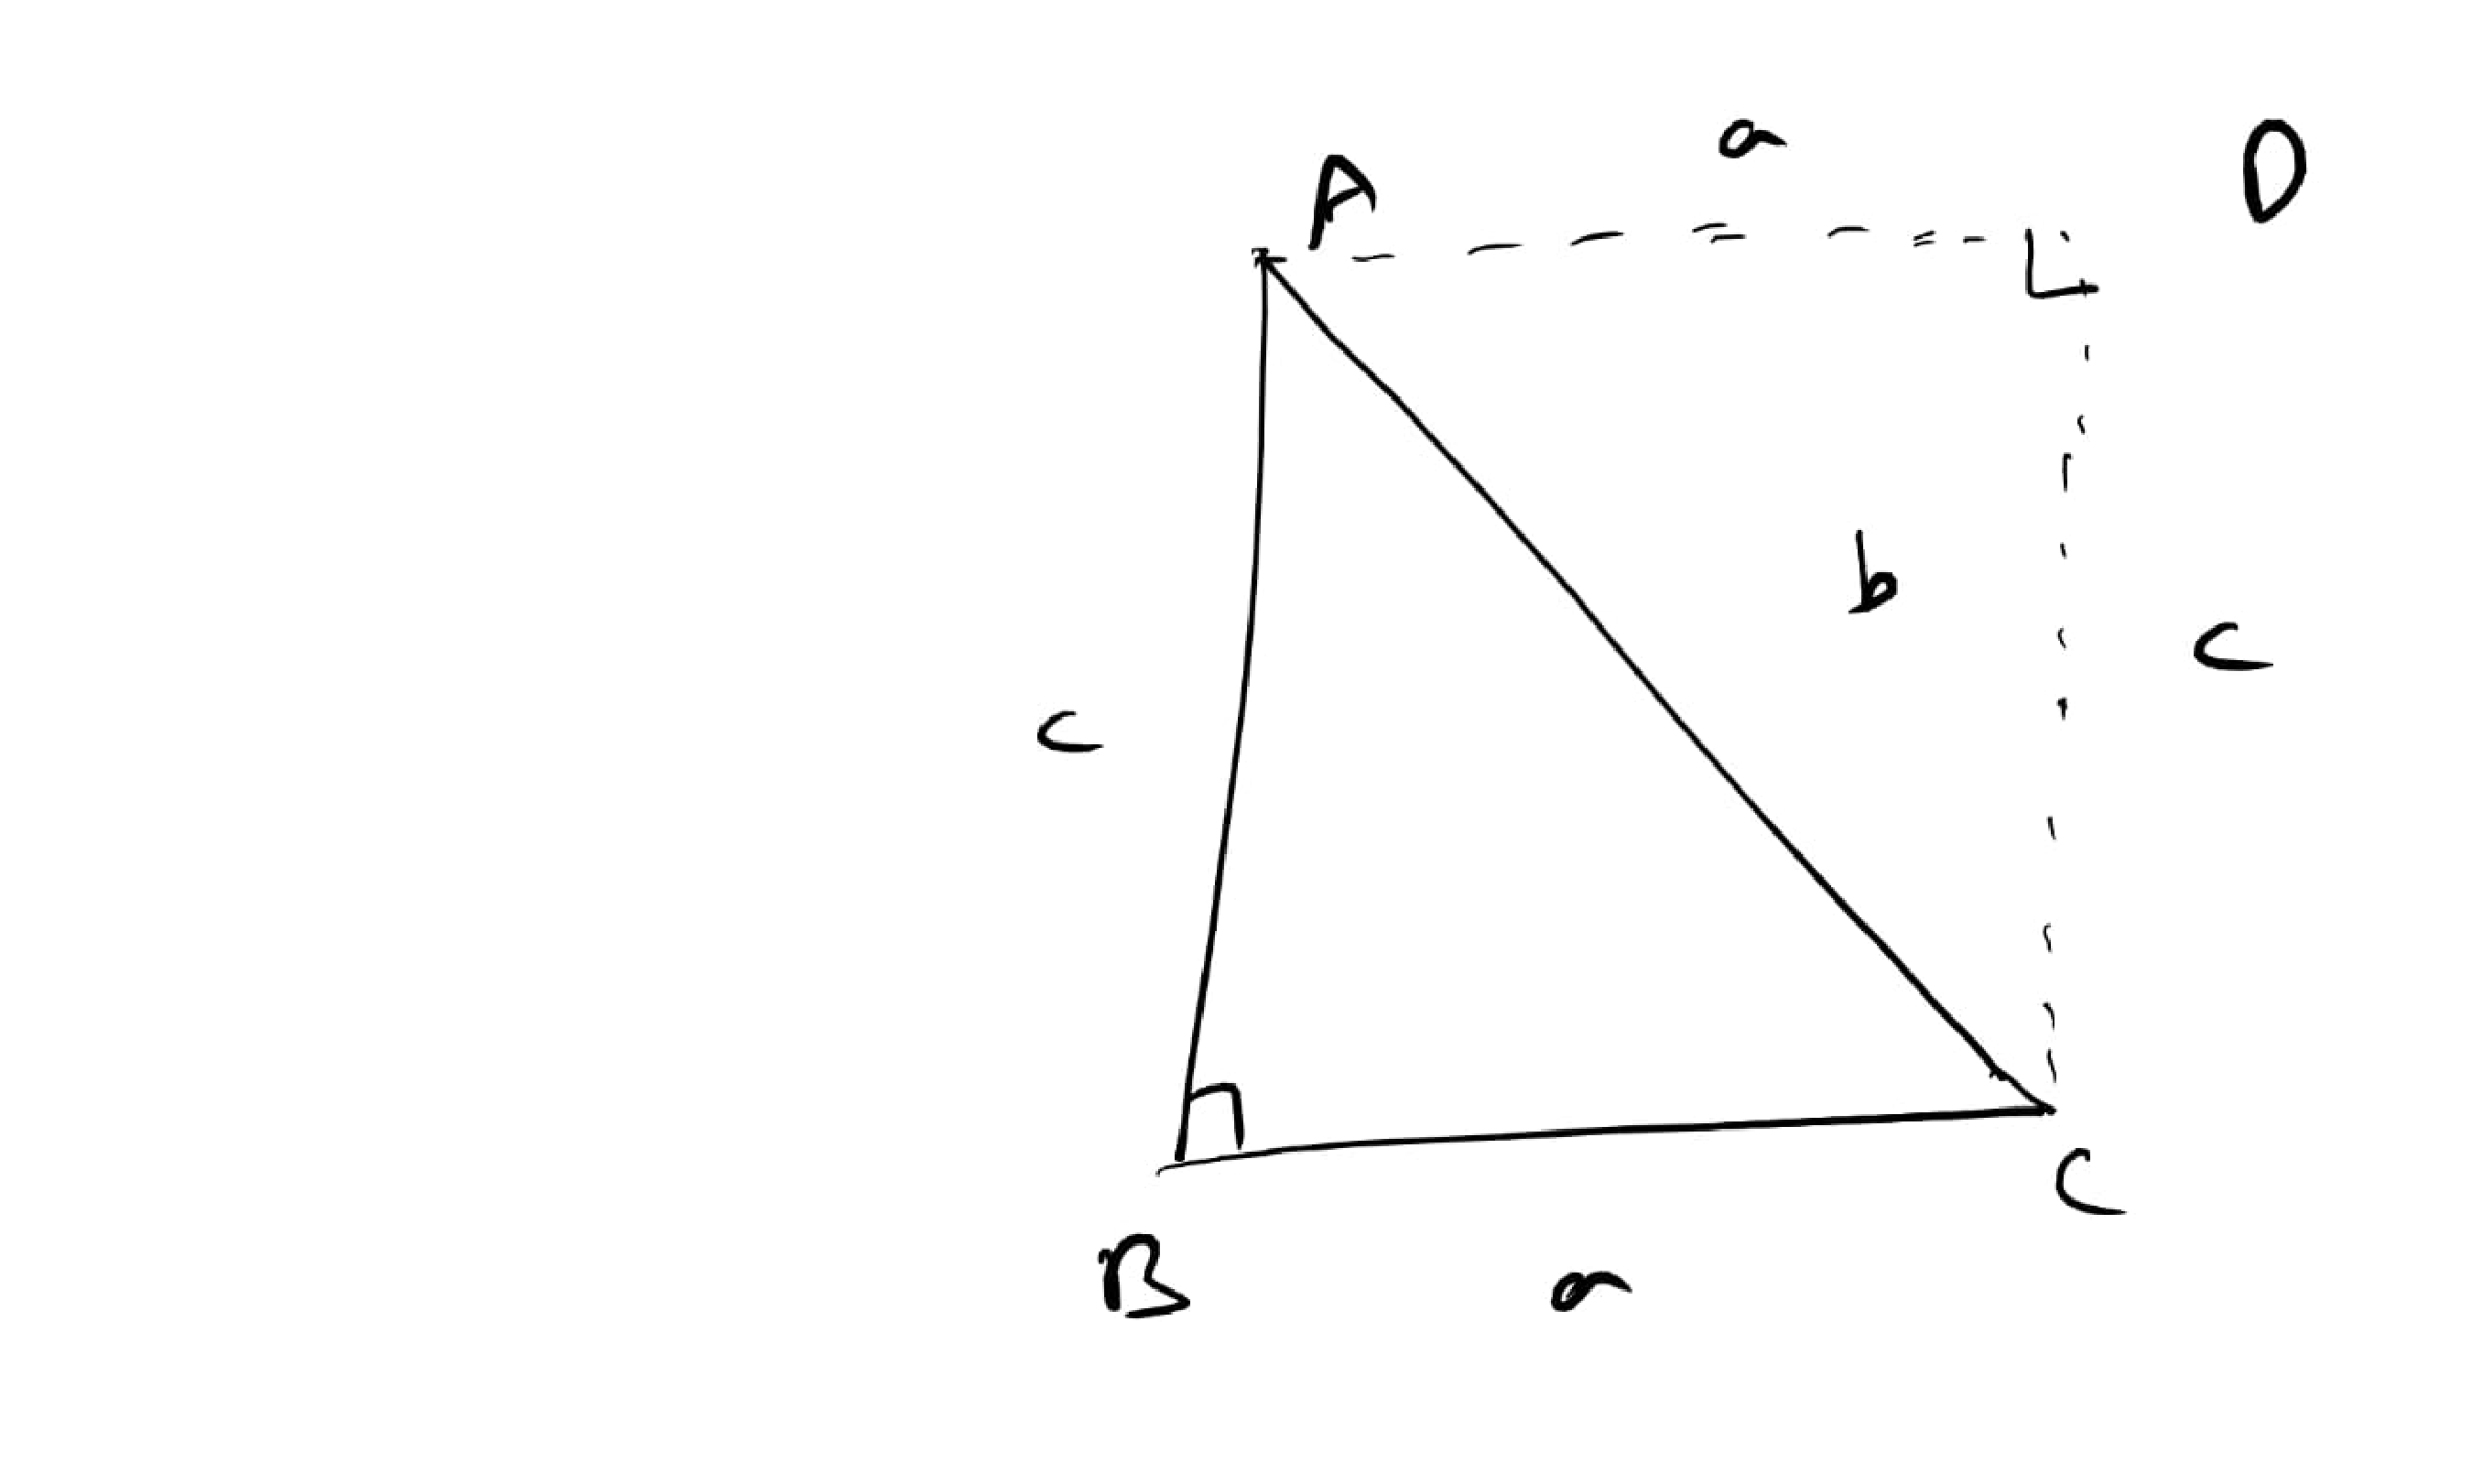
\includegraphics[width=\columnwidth]{./triangle/figs/tri_right_area.eps}
%\caption{}
%\label{fig:tri_right_area}
%\end{figure}
%%
%For any $\triangle ABC$, as shown in Fig.  \ref{fig:tri_area}, the area can be obtained as
%%
%\begin{align}
%\text{ar}\triangle ABC&=\frac{1}{2}xh+\frac{1}{2}yh 
%\\
%\frac{1}{2}\brak{x+y}h = \frac{1}{2}ah
%\end{align} 
%%

%
%\begin{figure}[!ht]
%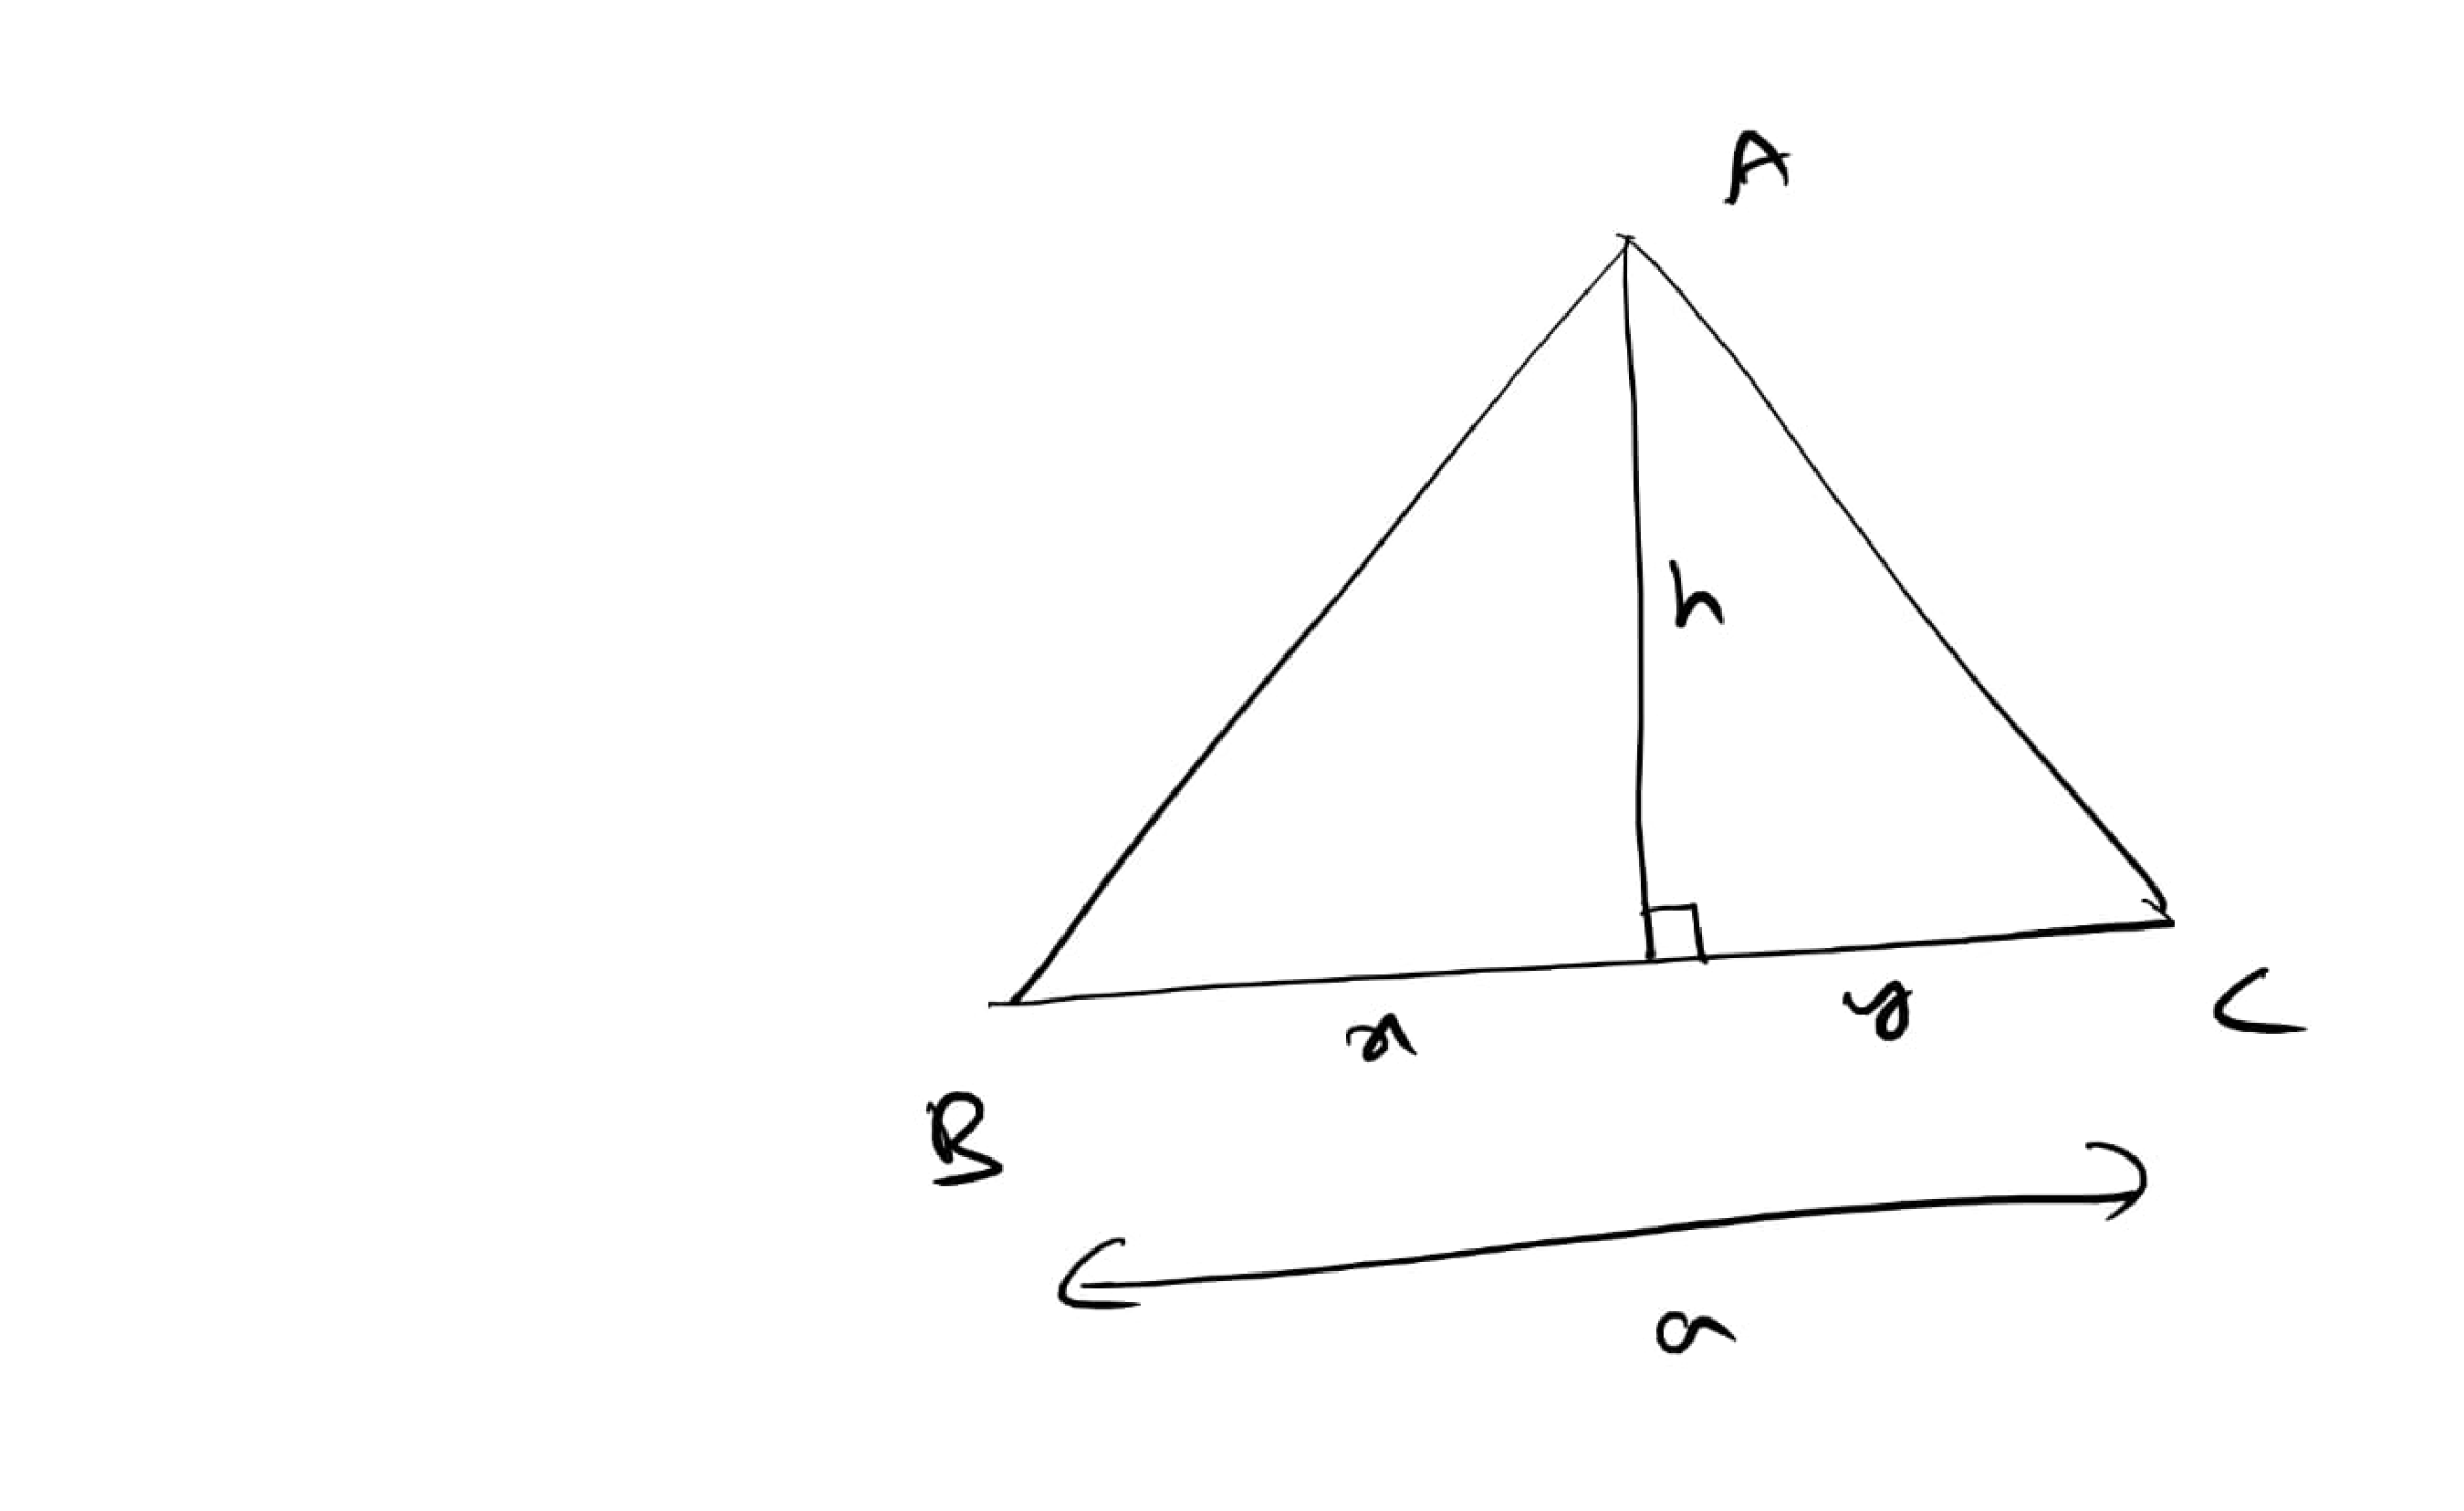
\includegraphics[width=\columnwidth]{./triangle/figs/tri_area.eps}
%\caption{}
%\label{fig:tri_area}
%\end{figure}
%
\item Find the area of a triangle whose vertices are 
$\vec{A}=\myvec{1\\-1}, 
\vec{B} = \myvec{-4\\6}$ and
$ 
\vec{C} = \myvec{-3\\-5}
$.
%
\\
\solution
  Using Hero's formula, the following code computes the area of the  triangle as 24.
%
\begin{lstlisting}
codes/triangle/area_tri.py
\end{lstlisting}
%
%\item A median of a triangle divides it into two triangles of equal areas.
%\\
%\solution In $\triangle ABC$, let $AD$
%
\item Find the area of a triangle formed by the vertices $\vec{A}=\myvec{5\\2}, \vec{B}=\myvec{4\\7}, \vec{C}=\myvec{7\\-4}$.
%\\
\solution  The area of $\triangle ABC$ is also obtained  in terms of the  {\em magnitude} of the determinant of the matrix $\vec{M}$ in  \eqref{eq:tri_geo_ex_diff_mat} as
%
\begin{align}
\frac{1}{2}\mydet{\vec{M}}
\end{align}
The computation is done in \textbf{area\_tri.py}
\item Find the area of a triangle formed by the points $\vec{P}=\myvec{-1.5\\3}, \vec{Q}=\myvec{6\\-2}, \vec{R}=\myvec{-3\\4}$.
\\
\solution Another formula for the area of $\triangle ABC$  is
%
\begin{align}
\frac{1}{2}\mydet{1 & 1 & 1\\ \vec{A} & \vec{B} & \vec{C} }
\end{align}
%
\item Find the area of a triangle having the points
%
\begin{align}
\vec{A} = \myvec{1\\1 \\1},
\vec{B} = \myvec{1\\2 \\3},
\vec{C} = \myvec{2\\ 3\\1}
\end{align}
%
as its vertices.
\\
\solution The area of a triangle using the {\em vector product} is obtained as
\begin{align}
\frac{1}{2}\norm{\brak{\vec{B}-\vec{A}}\times \brak{\vec{C}-\vec{A}}}
\end{align}
%
For any two vectors $\vec{a}=\myvec{a_1\\a_2\\a_3}, \vec{b}=\myvec{b_1\\b_2\\b_3}$, 
\begin{align}
\label{eq:tri_cross_prod}
\vec{a}\times \vec{b} = \myvec{0 & -a_3 & a_2 \\ a_3 & 0 & -a_1 \\ -a_2 & a_1 & 0}\myvec{b_1\\b_2\\b_3}
\end{align}
%
The following code computes the area using the vector product.
%
\begin{lstlisting}
codes/triangle/area_tri_vec.py
\end{lstlisting}
%
%
\item The centroid of a $\triangle ABC$ is at the point \myvec{1\\1\\1}.  If the coordinates of $\vec{A}$ and $\vec{B}$ are \myvec{3\\-5\\7} and \myvec{-1\\7\\-6}, respectively, find the coordinates of the point $\vec{C}$.
%
\\
\solution The centroid of $\triangle ABC$ is given by
\begin{align}
\label{eq:tri_geo_ex_centroid}
\vec{O} = \frac{\vec{A}+\vec{B}+\vec{C}}{3}
\end{align}
%
Thus, 
\begin{align}
\vec{C} = 3\vec{C}-\vec{A}-\vec{B}
\end{align}
%
\item Without using the Pythagoras theorem, show that the points \myvec{4\\ 4}, \myvec{3\\ 5} and \myvec{–1\\ –1} are the vertices of a right angled triangle.
\\
\solution
In general, the complex number $\myvec{a_1\\a_2}$ has the matrix representation
\begin{align}
\label{eq:3.4.1_Complex}
\myvec{a_1\\a_2} &= \myvec{a_1 & -a_2\\ a_2 & a_1}\myvec{1\\0}
\\
&= \vec{T}_a\myvec{1\\0}
\\
\implies \myvec{5\\-3}&=\myvec{5&3\\-3&5}\myvec{1\\0}
\end{align}
Then,
\begin{align}
\myvec{5\\-3}^3 &\triangleq\myvec{5&3\\-3&5}^3\myvec{1\\0}
\\
 &= \myvec{-10&198\\-198&-10} \myvec{1\\0}
\\
&=\myvec{-10\\-198}
\end{align}
The python code for above problem is
\begin{lstlisting}
codes/line/comp.py
\end{lstlisting}

\item Draw the graphs of the equations 
\begin{align}
\label{eq:1.2.1_p1}
\myvec{1 & -1}\vec{x} + 1 &= 0 
\\
\myvec{ 3 & 2}\vec{x} - 12 &= 0
\label{eq:1.2.1_p2}
\end{align}
%
 Determine the coordinates of the vertices of the triangle formed by these lines and the x-axis, and shade the triangular region.
\\
\solution
In general, the complex number $\myvec{a_1\\a_2}$ has the matrix representation
\begin{align}
\label{eq:3.4.1_Complex}
\myvec{a_1\\a_2} &= \myvec{a_1 & -a_2\\ a_2 & a_1}\myvec{1\\0}
\\
&= \vec{T}_a\myvec{1\\0}
\\
\implies \myvec{5\\-3}&=\myvec{5&3\\-3&5}\myvec{1\\0}
\end{align}
Then,
\begin{align}
\myvec{5\\-3}^3 &\triangleq\myvec{5&3\\-3&5}^3\myvec{1\\0}
\\
 &= \myvec{-10&198\\-198&-10} \myvec{1\\0}
\\
&=\myvec{-10\\-198}
\end{align}
The python code for above problem is
\begin{lstlisting}
codes/line/comp.py
\end{lstlisting}

%
\item In a $\triangle ABC, \angle C = 3 \angle B = 2 (\angle A + \angle B)$. Find the three angles. 
\\
\solution
In general, the complex number $\myvec{a_1\\a_2}$ has the matrix representation
\begin{align}
\label{eq:3.4.1_Complex}
\myvec{a_1\\a_2} &= \myvec{a_1 & -a_2\\ a_2 & a_1}\myvec{1\\0}
\\
&= \vec{T}_a\myvec{1\\0}
\\
\implies \myvec{5\\-3}&=\myvec{5&3\\-3&5}\myvec{1\\0}
\end{align}
Then,
\begin{align}
\myvec{5\\-3}^3 &\triangleq\myvec{5&3\\-3&5}^3\myvec{1\\0}
\\
 &= \myvec{-10&198\\-198&-10} \myvec{1\\0}
\\
&=\myvec{-10\\-198}
\end{align}
The python code for above problem is
\begin{lstlisting}
codes/line/comp.py
\end{lstlisting}

\item Draw the graphs of the equations $5x – y = 5$ and $3x – y = 3$. Determine the co-ordinates of the vertices of the triangle formed by these lines and the y axis.
\\
\solution
In general, the complex number $\myvec{a_1\\a_2}$ has the matrix representation
\begin{align}
\label{eq:3.4.1_Complex}
\myvec{a_1\\a_2} &= \myvec{a_1 & -a_2\\ a_2 & a_1}\myvec{1\\0}
\\
&= \vec{T}_a\myvec{1\\0}
\\
\implies \myvec{5\\-3}&=\myvec{5&3\\-3&5}\myvec{1\\0}
\end{align}
Then,
\begin{align}
\myvec{5\\-3}^3 &\triangleq\myvec{5&3\\-3&5}^3\myvec{1\\0}
\\
 &= \myvec{-10&198\\-198&-10} \myvec{1\\0}
\\
&=\myvec{-10\\-198}
\end{align}
The python code for above problem is
\begin{lstlisting}
codes/line/comp.py
\end{lstlisting}


\item The vertices of $\triangle PQR$ are 

$
\vec{P} = \myvec{2 \\1},
\vec{Q} = \myvec{-2\\3},
\vec{R} = \myvec{4\\5}.
$
Find the equation of the median through the vertex $\vec{R}$.
\\
\solution
In general, the complex number $\myvec{a_1\\a_2}$ has the matrix representation
\begin{align}
\label{eq:3.4.1_Complex}
\myvec{a_1\\a_2} &= \myvec{a_1 & -a_2\\ a_2 & a_1}\myvec{1\\0}
\\
&= \vec{T}_a\myvec{1\\0}
\\
\implies \myvec{5\\-3}&=\myvec{5&3\\-3&5}\myvec{1\\0}
\end{align}
Then,
\begin{align}
\myvec{5\\-3}^3 &\triangleq\myvec{5&3\\-3&5}^3\myvec{1\\0}
\\
 &= \myvec{-10&198\\-198&-10} \myvec{1\\0}
\\
&=\myvec{-10\\-198}
\end{align}
The python code for above problem is
\begin{lstlisting}
codes/line/comp.py
\end{lstlisting}

\item In the $\triangle ABC$ with vertices
$
\vec{A}=\myvec{2\\3}, 
\vec{B}=\myvec{4\\-1},
 \vec{C}=\myvec{1\\2}
$,
find the equation and length of the altitude from the vertex $\vec{A}$.
\\
\solution
	The following python code computes the length of the altitude $\vec{AD}$ in Fig.\ref{fig:1.2.5_qtwo}.
	\begin{lstlisting}
	./solutions/5/codes/triangle/q2.py
	\end{lstlisting}
	
	\begin{figure}[!ht]
	\centering
	\includegraphics[width=\columnwidth]{./solutions/5/figs/triangle/q2.eps}
	\caption{Triangle of Q.1.2.5}
	\label{fig:1.2.5_qtwo}	
	\end{figure}
	
In $\triangle ABC$, 
	\begin{align}
\brak{\vec{A}-\vec{C}}^T\brak{\vec{B}-\vec{C}} = 0
	\end{align}
Hence, $ABC$ is a right triangle. The direction vector of $BC$ is 
\begin{align}
\brak{\vec{B}-\vec{C}} = \myvec{3\\-3}
\end{align}
Hence, the equation of $AD$ is 
\begin{align}
\brak{\vec{B}-\vec{C}}^T \brak{\vec{x}-\vec{A}} &= 0
\\
\implies 		\myvec{1&-1}\vec{x} &= -1
\end{align}
The length of the altitude is obtained as $\norm{\vec{A-D}} = 1.414$
	
	
	
	

\item Find the area of the triangle whose vertices are
\begin{enumerate}
\item \myvec{2\\3}, \myvec{-1\\0},  \myvec{2\\-4}
\item  \myvec{-5\\-1},  \myvec{3\\-5},  \myvec{5\\2}
\end{enumerate}
\solution
In general, the complex number $\myvec{a_1\\a_2}$ has the matrix representation
\begin{align}
\label{eq:3.4.1_Complex}
\myvec{a_1\\a_2} &= \myvec{a_1 & -a_2\\ a_2 & a_1}\myvec{1\\0}
\\
&= \vec{T}_a\myvec{1\\0}
\\
\implies \myvec{5\\-3}&=\myvec{5&3\\-3&5}\myvec{1\\0}
\end{align}
Then,
\begin{align}
\myvec{5\\-3}^3 &\triangleq\myvec{5&3\\-3&5}^3\myvec{1\\0}
\\
 &= \myvec{-10&198\\-198&-10} \myvec{1\\0}
\\
&=\myvec{-10\\-198}
\end{align}
The python code for above problem is
\begin{lstlisting}
codes/line/comp.py
\end{lstlisting}


\item Find the area of the triangle formed by joining the mid points of the sides of a triangle whose vertices are  \myvec{0\\-1},  \myvec{2\\1},  \myvec{0\\3}.
\\
\solution
In general, the complex number $\myvec{a_1\\a_2}$ has the matrix representation
\begin{align}
\label{eq:3.4.1_Complex}
\myvec{a_1\\a_2} &= \myvec{a_1 & -a_2\\ a_2 & a_1}\myvec{1\\0}
\\
&= \vec{T}_a\myvec{1\\0}
\\
\implies \myvec{5\\-3}&=\myvec{5&3\\-3&5}\myvec{1\\0}
\end{align}
Then,
\begin{align}
\myvec{5\\-3}^3 &\triangleq\myvec{5&3\\-3&5}^3\myvec{1\\0}
\\
 &= \myvec{-10&198\\-198&-10} \myvec{1\\0}
\\
&=\myvec{-10\\-198}
\end{align}
The python code for above problem is
\begin{lstlisting}
codes/line/comp.py
\end{lstlisting}

\item Verify that the median of $\triangle ABC$ with vertices $\vec{A}=\myvec{4\\-6},  \vec{B}=\myvec{3\\-2}$ and  $\vec{C} =  \myvec{5\\2}$ divides it into two triangles of equal areas.
\\
\solution
In general, the complex number $\myvec{a_1\\a_2}$ has the matrix representation
\begin{align}
\label{eq:3.4.1_Complex}
\myvec{a_1\\a_2} &= \myvec{a_1 & -a_2\\ a_2 & a_1}\myvec{1\\0}
\\
&= \vec{T}_a\myvec{1\\0}
\\
\implies \myvec{5\\-3}&=\myvec{5&3\\-3&5}\myvec{1\\0}
\end{align}
Then,
\begin{align}
\myvec{5\\-3}^3 &\triangleq\myvec{5&3\\-3&5}^3\myvec{1\\0}
\\
 &= \myvec{-10&198\\-198&-10} \myvec{1\\0}
\\
&=\myvec{-10\\-198}
\end{align}
The python code for above problem is
\begin{lstlisting}
codes/line/comp.py
\end{lstlisting}

\item Let $\vec{A}=\myvec{4\\2},  \vec{B}=\myvec{6\\5}$ and  $\vec{C} =  \myvec{1\\4}$ be the vertices of $\triangle ABC$.
\begin{enumerate}
\item The median from $\vec{A}$ meets $BC$ at $\vec{D}$.  Find the coordinates of the point $\vec{D}$.
\item Find the coordinates of the point $\vec{P}$ on $AD$ such that $AP:PD = 2:1$.
\item Find the coordinates of the points $\vec{Q}$ and $\vec{R}$ on medians $BE$ and $CF$ respectively such that $BQ:QE = 2:1$ and $CR:RF = 2:1$.
\end{enumerate}
\solution



\begin{figure}[!ht]
    \centering
    \includegraphics[width=\columnwidth]{solutions/su2021/2/56/Figure9_1.png}
    \caption{Inequality pair 1}
    \label{ineq/56/fig:inequalities1}	
    \end{figure}
    
    \begin{figure}[!ht]
    \centering
    \includegraphics[width=\columnwidth]{solutions/su2021/2/56/Figure9_2.png}
    \caption{Inequality pair 2}
    \label{ineq/56/fig:inequalities2}	
    \end{figure}
    
    \begin{figure}[!ht]
    \centering
    \includegraphics[width=\columnwidth]{solutions/su2021/2/56/Figure 9_3.png}
    \caption{Intersection of \ref{ineq/56/fig:inequalities1} and \ref{ineq/56/fig:inequalities2}}
    \label{ineq/56/fig:inequality3}	
    \end{figure}
    The common region shown by \ref{ineq/56/fig:inequality3} is the solution of set of inequalities.
    
\item Show that the points 
\begin{align}
\vec{A} = \myvec{2\\-1 \\1},
\vec{B} = \myvec{1\\-3 \\-5},
\vec{C} = \myvec{3\\ -4\\-4}
\end{align}
%
are the vertices of a right angled triangle.
\\
\solution

\begin{align}
\because \myvec{\vec{A-C}}^\top\myvec{\vec{B-C}}=\myvec{-1&3&5}\myvec{-2\\1\\-1}\\=0
\end{align}
the triangle in Fig.     \ref{fig:vec/2/4/} is right angled.
\begin{figure}[ht]
    \centering
    \includegraphics[width=\columnwidth]{solutions/su2021/2/4/Right angle triangle.png}
    \caption{}
    \label{fig:vec/2/4/}
    \end{figure} 




\item In $\triangle ABC$, 
$
\vec{A} = \myvec{1\\2 \\3},
\vec{B} = \myvec{-1\\0 \\0},
\vec{C} = \myvec{0\\ 1\\2}.
$
Find $\angle B$.
\\
\solution
Data from the given question is available in Table \ref{constr/circ/61/tab:table1}:
%
\begin{table}[!ht]
\begin{center}
\begin{tabular}{ | m{2cm} | m{1.5cm}| m{2cm} | m{1.5cm} |} 
\hline
& Symbols & Circle1  \\
\hline
Centre & $\vec{C}$ & \myvec{0\\0}  \\ 
\hline
Radius & $r$& 3.4 \\ 
\hline
\end{tabular}
\end{center}
\caption{Input values}
\label{constr/circ/61/tab:table1}
\end{table}
%
Let 
\begin{align}
      \vec{P} &= r \myvec{\cos \theta_1\\ \sin \theta_1} =  \myvec{1.7\\2.9}
      \\
      \vec{Q} &= r \myvec{\cos \theta_2\\ \sin \theta_2} =\myvec{-2.4\\2.4}
 \end{align}
 Then the perpendicular bisector of $PQ$ passes through 
 \begin{align}
    \vec{M} = \frac{\vec{P}+\vec{Q}}{2} 
\end{align}
and has normal vector 
\begin{align}
    \vec{n} = \vec{P}-\vec{Q}
\end{align}
resulting in the equation
\begin{align}
    \brak{\vec{P}-\vec{Q}}^\top\brak{\vec{x}-\frac{\vec{P}+\vec{Q}}{2} } = 0
    \implies \brak{\vec{P}-\vec{Q}}^\top\vec{x} = 0
\end{align}
%
after simplification.  It is obvious that $\vec{O}$ satisfies the above equuation as can be verified in Fig.     \ref{constr/circ/61/fig: perpenicular bisector of the chord passes through the center}.
%
\begin{figure}[ht]
    \centering
    \includegraphics[width=\columnwidth]{solutions/circle/61/FIG.3.png}
    \caption{perpendicular bisector of the chord passes through the center}
    \label{constr/circ/61/fig: perpenicular bisector of the chord passes through the center}
\end{figure}







\item Find the area of a triangle having the points 
$
\vec{A} = \myvec{1\\1 \\1},
\vec{B} = \myvec{1\\2 \\3}, \text{ and }
\vec{C} = \myvec{2\\ 3\\1}
$
as its vertices.
\\
\solution
From the given information, 
%
\begin{align}
    \vec{B-A}=\myvec{1\\2\\3}-\myvec{1\\1\\1} = \myvec{0\\1\\2}\\
    \vec{C-A}=\myvec{2\\3\\1}-\myvec{1\\1\\1}=\myvec{1\\2\\0}\\
    \end{align}
The area of a triangle using the vector product is then obtained as
\begin{align}
    \frac{1}{2}\norm{\myvec{\vec{B-A}}\times\myvec{\vec{C-A}}}\\ \frac{1}{2}\norm{\myvec{0\\1\\2}\times \myvec{1\\2\\0}}\\=1
    \end{align}
%
\item Find the area of a triangle with vertices
$
\vec{A} = \myvec{1\\1 \\2},
\vec{B} = \myvec{2\\3 \\5}, \text{ and }
\vec{C} = \myvec{1\\ 5\\5}
$
\\
\solution
From the given information, 
%
\begin{align}
\vec{B-A}&=\myvec{2\\3\\5}-\myvec{1\\1\\2} = \myvec{1\\2\\3}\\
\vec{C-A}&=\myvec{1\\5\\5}-\myvec{1\\1\\2}=\myvec{0\\4\\3}
\end{align}
The area of a triangle using the vector product is then obtained as
\begin{align}
        \frac{1}{2}\norm{\myvec{\vec{B-A}}\times\myvec{\vec{C-A}}} \\=\frac{1}{2}\norm{\myvec{1\\2\\3}\times \myvec{0\\4\\3}}\\=\frac{17}{2}
    \end{align}
\item Show that 
$
\vec{A}=\myvec{2\\3\\-4}, 
\vec{B}=\myvec{1\\-2\\3} \text{ and } 
\vec{C}=\myvec{3\\8\\-11}$  
are collinear.
\\
\solution 
%
Data from the given question is available in Table \ref{constr/circ/61/tab:table1}:
%
\begin{table}[!ht]
\begin{center}
\begin{tabular}{ | m{2cm} | m{1.5cm}| m{2cm} | m{1.5cm} |} 
\hline
& Symbols & Circle1  \\
\hline
Centre & $\vec{C}$ & \myvec{0\\0}  \\ 
\hline
Radius & $r$& 3.4 \\ 
\hline
\end{tabular}
\end{center}
\caption{Input values}
\label{constr/circ/61/tab:table1}
\end{table}
%
Let 
\begin{align}
      \vec{P} &= r \myvec{\cos \theta_1\\ \sin \theta_1} =  \myvec{1.7\\2.9}
      \\
      \vec{Q} &= r \myvec{\cos \theta_2\\ \sin \theta_2} =\myvec{-2.4\\2.4}
 \end{align}
 Then the perpendicular bisector of $PQ$ passes through 
 \begin{align}
    \vec{M} = \frac{\vec{P}+\vec{Q}}{2} 
\end{align}
and has normal vector 
\begin{align}
    \vec{n} = \vec{P}-\vec{Q}
\end{align}
resulting in the equation
\begin{align}
    \brak{\vec{P}-\vec{Q}}^\top\brak{\vec{x}-\frac{\vec{P}+\vec{Q}}{2} } = 0
    \implies \brak{\vec{P}-\vec{Q}}^\top\vec{x} = 0
\end{align}
%
after simplification.  It is obvious that $\vec{O}$ satisfies the above equuation as can be verified in Fig.     \ref{constr/circ/61/fig: perpenicular bisector of the chord passes through the center}.
%
\begin{figure}[ht]
    \centering
    \includegraphics[width=\columnwidth]{solutions/circle/61/FIG.3.png}
    \caption{perpendicular bisector of the chord passes through the center}
    \label{constr/circ/61/fig: perpenicular bisector of the chord passes through the center}
\end{figure}







\item Find the equation of set of points $\vec{P}$ such that
\begin{align}
PA^2+PB^2 =2k^2,
\end{align}
%
\begin{align}
\vec{A} = \myvec{3\\4 \\5},
\vec{B} = \myvec{-1\\3 \\-7},
\end{align}
%
respectively.
%
%
\solution
\begin{enumerate}
    \item Given that
    \begin{align}
    \vec{A} = \myvec{1 & -1 \\ 2 & 3}
    \end{align}
    The augmented matrix $ [A | I]$ is as given below:- 
    \begin{align}
    \myvec{1 & -1 & \vrule & 1 & 0 \\ 2 & 3 & \vrule & 0 & 1}
    \end{align}
    We apply the elementary row operations on $ [A | I]$ as follows :-
    \begin{align}
    [A | I] = \myvec{1 & -1 & \vrule & 1 & 0 \\ 2 & 3 & \vrule & 0 & 1}
    \\
    \xleftrightarrow{R_2\leftarrow R_2-2R_1}   
    \myvec{1 & -1 & \vrule & 1 & 0 \\ 0 & 5 & \vrule & -2 & 1}
    \\
    \xleftrightarrow{R_2\leftarrow \frac{R_2}{5}}
    \myvec{1 & -1 & \vrule & 1 & 0 \\ 0 & 1 & \vrule & \frac {-2}{5} & \frac {1}{5}}
    \\
    \xleftrightarrow{R_2\leftarrow R_1+R_2}
    \myvec{1 & 0 & \vrule & \frac{3}{5} & \frac{1}{5} \\ 0 & 1 & \vrule & \frac{-2}{5} & \frac{1}{5}}
    \end{align}
    By performing elementary transformations on augmented matrix$ [A | I]$ , we obtained the augmented matrix in the form $ [I | A]$. 
    Hence we can conclude that the matrix A is invertible and inverse of the matrix is:-
    \begin{align}
    \therefore\vec{A^{-1}}=\myvec {\frac{3}{5} & \frac{1}{5} \\  \frac{-2}{5} & \frac{1}{5}} 
    \end{align}
    \item QR decomposition of  \myvec{1 & -1 \\ 2 & 3}
    \begin{align}
    \vec{v_1}=\myvec{1 \\ 2},
    \vec{v_2}=\myvec{-1 \\ 3}
    \end{align}
    \begin{align}
    \vec{r_1{}_1}&=\sqrt{5}
    \\
    \vec{q_1}&=\frac{1}{\norm{\vec{v_1}}}{\vec{v_1}}=\myvec{\frac{1}{\sqrt{5}} \\ \frac{2}{\sqrt{5}}}
    \\
    \vec{r_1{}_2}&=\vec{v_1}^{T}{\vec{v_2}} 
    \\
    &=\myvec{\frac{1}{\sqrt{5}} & \frac{1}{\sqrt{5}}}\myvec{-1 \\ 3 }=\sqrt{5}
    \\
    \vec{v_2}&=\vec{v_2}-\vec{r_1{}_2}\vec{q_1} \\
    &=\myvec{-1 \\ 3}-{\sqrt{5}}\myvec{\frac{1}{\sqrt{5}} \\ \frac{1}{\sqrt{5}}}
    \\
    &=\myvec{-2 \\ 1}
    \\
    \vec{r_2{}_2}&=\norm{\vec{v_2}}=\sqrt{5}
    \\
    \vec{q_2}&=\frac{1}{\norm{v_2}}\vec{v_2}
    \\
    &=\frac{1}{\sqrt{5}}\myvec{\frac{-2}{\sqrt{5}} \\ \frac{1}{\sqrt{5}}}=\myvec{\frac{-2}{\sqrt{5}}\\{\frac{1}{\sqrt{5}}}}
    \end{align}
    Thus obtained QR decomposition is 
    \begin{align}
    \myvec{1 & -1 \\ 2 & 3}=\myvec{\frac{1}{\sqrt{5}} & \frac{-2}{\sqrt{5}} \\ \frac{2}{\sqrt{5}} & \frac{1}{\sqrt{5}}}\myvec{\sqrt{5} & \sqrt{5} \\ 0 & \sqrt{5}}
    \end{align}
    \end{enumerate}   

\item Find the coordinates of a point which divides the line segment joining the points \myvec{1\\-2\\3} and \myvec{3\\4\\-5} in the ratio $2:3$
\begin{enumerate}
\item internally, and
\item externally.
\end{enumerate}
%
\solution
Data from the given question is available in Table \ref{constr/circ/61/tab:table1}:
%
\begin{table}[!ht]
\begin{center}
\begin{tabular}{ | m{2cm} | m{1.5cm}| m{2cm} | m{1.5cm} |} 
\hline
& Symbols & Circle1  \\
\hline
Centre & $\vec{C}$ & \myvec{0\\0}  \\ 
\hline
Radius & $r$& 3.4 \\ 
\hline
\end{tabular}
\end{center}
\caption{Input values}
\label{constr/circ/61/tab:table1}
\end{table}
%
Let 
\begin{align}
      \vec{P} &= r \myvec{\cos \theta_1\\ \sin \theta_1} =  \myvec{1.7\\2.9}
      \\
      \vec{Q} &= r \myvec{\cos \theta_2\\ \sin \theta_2} =\myvec{-2.4\\2.4}
 \end{align}
 Then the perpendicular bisector of $PQ$ passes through 
 \begin{align}
    \vec{M} = \frac{\vec{P}+\vec{Q}}{2} 
\end{align}
and has normal vector 
\begin{align}
    \vec{n} = \vec{P}-\vec{Q}
\end{align}
resulting in the equation
\begin{align}
    \brak{\vec{P}-\vec{Q}}^\top\brak{\vec{x}-\frac{\vec{P}+\vec{Q}}{2} } = 0
    \implies \brak{\vec{P}-\vec{Q}}^\top\vec{x} = 0
\end{align}
%
after simplification.  It is obvious that $\vec{O}$ satisfies the above equuation as can be verified in Fig.     \ref{constr/circ/61/fig: perpenicular bisector of the chord passes through the center}.
%
\begin{figure}[ht]
    \centering
    \includegraphics[width=\columnwidth]{solutions/circle/61/FIG.3.png}
    \caption{perpendicular bisector of the chord passes through the center}
    \label{constr/circ/61/fig: perpenicular bisector of the chord passes through the center}
\end{figure}







%\solution Use \eqref{eq:line_section_form}.

\item Prove that the three points \myvec{-4\\6\\10}, \myvec{2\\4\\6} and \myvec{14\\0\\-2} are collinear.
%
\\
\solution 
%
Data from the given question is available in Table \ref{constr/circ/61/tab:table1}:
%
\begin{table}[!ht]
\begin{center}
\begin{tabular}{ | m{2cm} | m{1.5cm}| m{2cm} | m{1.5cm} |} 
\hline
& Symbols & Circle1  \\
\hline
Centre & $\vec{C}$ & \myvec{0\\0}  \\ 
\hline
Radius & $r$& 3.4 \\ 
\hline
\end{tabular}
\end{center}
\caption{Input values}
\label{constr/circ/61/tab:table1}
\end{table}
%
Let 
\begin{align}
      \vec{P} &= r \myvec{\cos \theta_1\\ \sin \theta_1} =  \myvec{1.7\\2.9}
      \\
      \vec{Q} &= r \myvec{\cos \theta_2\\ \sin \theta_2} =\myvec{-2.4\\2.4}
 \end{align}
 Then the perpendicular bisector of $PQ$ passes through 
 \begin{align}
    \vec{M} = \frac{\vec{P}+\vec{Q}}{2} 
\end{align}
and has normal vector 
\begin{align}
    \vec{n} = \vec{P}-\vec{Q}
\end{align}
resulting in the equation
\begin{align}
    \brak{\vec{P}-\vec{Q}}^\top\brak{\vec{x}-\frac{\vec{P}+\vec{Q}}{2} } = 0
    \implies \brak{\vec{P}-\vec{Q}}^\top\vec{x} = 0
\end{align}
%
after simplification.  It is obvious that $\vec{O}$ satisfies the above equuation as can be verified in Fig.     \ref{constr/circ/61/fig: perpenicular bisector of the chord passes through the center}.
%
\begin{figure}[ht]
    \centering
    \includegraphics[width=\columnwidth]{solutions/circle/61/FIG.3.png}
    \caption{perpendicular bisector of the chord passes through the center}
    \label{constr/circ/61/fig: perpenicular bisector of the chord passes through the center}
\end{figure}







\item Find the equation of the set of points $\vec{P}$ such that its distances from the points
$
\vec{A}=\myvec{3\\4\\-5}, 
\vec{B}=\myvec{-2\\1\\4}
$
are equal. 
\\
\solution
Data from the given question is available in Table \ref{constr/circ/61/tab:table1}:
%
\begin{table}[!ht]
\begin{center}
\begin{tabular}{ | m{2cm} | m{1.5cm}| m{2cm} | m{1.5cm} |} 
\hline
& Symbols & Circle1  \\
\hline
Centre & $\vec{C}$ & \myvec{0\\0}  \\ 
\hline
Radius & $r$& 3.4 \\ 
\hline
\end{tabular}
\end{center}
\caption{Input values}
\label{constr/circ/61/tab:table1}
\end{table}
%
Let 
\begin{align}
      \vec{P} &= r \myvec{\cos \theta_1\\ \sin \theta_1} =  \myvec{1.7\\2.9}
      \\
      \vec{Q} &= r \myvec{\cos \theta_2\\ \sin \theta_2} =\myvec{-2.4\\2.4}
 \end{align}
 Then the perpendicular bisector of $PQ$ passes through 
 \begin{align}
    \vec{M} = \frac{\vec{P}+\vec{Q}}{2} 
\end{align}
and has normal vector 
\begin{align}
    \vec{n} = \vec{P}-\vec{Q}
\end{align}
resulting in the equation
\begin{align}
    \brak{\vec{P}-\vec{Q}}^\top\brak{\vec{x}-\frac{\vec{P}+\vec{Q}}{2} } = 0
    \implies \brak{\vec{P}-\vec{Q}}^\top\vec{x} = 0
\end{align}
%
after simplification.  It is obvious that $\vec{O}$ satisfies the above equuation as can be verified in Fig.     \ref{constr/circ/61/fig: perpenicular bisector of the chord passes through the center}.
%
\begin{figure}[ht]
    \centering
    \includegraphics[width=\columnwidth]{solutions/circle/61/FIG.3.png}
    \caption{perpendicular bisector of the chord passes through the center}
    \label{constr/circ/61/fig: perpenicular bisector of the chord passes through the center}
\end{figure}







\item The line through the points \myvec{-2\\6} and \myvec{4\\8} is perpendicular to the line through the points \myvec{8\\12} and $\myvec{x\\24}$.  Find the value of $x$.
\\
\solution
Data from the given question is available in Table \ref{constr/circ/61/tab:table1}:
%
\begin{table}[!ht]
\begin{center}
\begin{tabular}{ | m{2cm} | m{1.5cm}| m{2cm} | m{1.5cm} |} 
\hline
& Symbols & Circle1  \\
\hline
Centre & $\vec{C}$ & \myvec{0\\0}  \\ 
\hline
Radius & $r$& 3.4 \\ 
\hline
\end{tabular}
\end{center}
\caption{Input values}
\label{constr/circ/61/tab:table1}
\end{table}
%
Let 
\begin{align}
      \vec{P} &= r \myvec{\cos \theta_1\\ \sin \theta_1} =  \myvec{1.7\\2.9}
      \\
      \vec{Q} &= r \myvec{\cos \theta_2\\ \sin \theta_2} =\myvec{-2.4\\2.4}
 \end{align}
 Then the perpendicular bisector of $PQ$ passes through 
 \begin{align}
    \vec{M} = \frac{\vec{P}+\vec{Q}}{2} 
\end{align}
and has normal vector 
\begin{align}
    \vec{n} = \vec{P}-\vec{Q}
\end{align}
resulting in the equation
\begin{align}
    \brak{\vec{P}-\vec{Q}}^\top\brak{\vec{x}-\frac{\vec{P}+\vec{Q}}{2} } = 0
    \implies \brak{\vec{P}-\vec{Q}}^\top\vec{x} = 0
\end{align}
%
after simplification.  It is obvious that $\vec{O}$ satisfies the above equuation as can be verified in Fig.     \ref{constr/circ/61/fig: perpenicular bisector of the chord passes through the center}.
%
\begin{figure}[ht]
    \centering
    \includegraphics[width=\columnwidth]{solutions/circle/61/FIG.3.png}
    \caption{perpendicular bisector of the chord passes through the center}
    \label{constr/circ/61/fig: perpenicular bisector of the chord passes through the center}
\end{figure}







\item Show that the line joining the origin to the point \myvec{2\\1\\1} is perpendicular to the line determined by the points \myvec{3\\5\\-1}, \myvec{4\\3\\-1}.
\\
\solution
Let 
\begin{align}
 \vec{O}=\myvec{0\\0\\0}, 
 \vec{P}=\myvec{2\\1\\1} ,\vec{A}=\myvec{3\\5\\-1} ,\vec{B}=\myvec{4\\3\\-1}  
\end{align}
Then,
\begin{align}
\vec{O}-\vec{P}&=\myvec{2\\1\\1}
\\
&=\myvec{4\\3\\-1}-\myvec{3\\5\\-1}
\\
\vec{A}-\vec{B}&=\myvec{1\\-2\\0}
\end{align}
and 
\begin{align}
\brak{\vec{O}-\vec{P}}^T(\vec{A}-\vec{B})=0
\\
\implies \brak{\vec{O}-\vec{P}} \perp \brak{\vec{A}-\vec{B}}
\end{align}
\item Are the points 
\begin{align}
\vec{A} = \myvec{3\\6 \\9},
\vec{B} = \myvec{10\\20 \\30},
\vec{C} = \myvec{25\\ -41\\5},
\end{align}
%
the vertices of a right angled triangle?
\\
\solution
Let
\begin{align}
   \vec{A} = \myvec{3\\6\\9} , \vec{B} = \myvec{10\\20\\30}, \vec{C} = \myvec{25\\-41\\5} 
\end{align}

\begin{align}
     (\vec{B}-\vec{A})^\top(\vec{C}-\vec{A})&=\myvec{7\ 14\ 21}\myvec{22\\-47\\-4}
     \\
& = -521 \ne 0
\\
     (\vec{A}-\vec{B})^\top(\vec{C}-\vec{B})&=\myvec{-7\ -14\ -21}\myvec{15\\-61\\-25}
\\
&= 1274 \ne 0
\\
(\vec{A}-\vec{B})^\top(\vec{C}-\vec{B})&=\myvec{-7\ -14\ -21}\myvec{15\\-61\\-25}
\\
&= 3397 \ne 0 
\end{align}
Hence, $\triangle ABC$ is not right angled as can be seen in Fig.          \ref{vectors/july/2/6/Figure}.
%
\begin{figure}[!h]
         \centering
         \includegraphics[width=\columnwidth]{solutions/july/2/6/Figures/Figure.png}
         \caption{Plot of the triangle}
         \label{vectors/july/2/6/Figure}
\end{figure}

\item Find a condition on $\vec{x}$  such that the points $\vec{x}, \myvec{1\\2}, \myvec{7\\0}$ are collinear.
\\
\solution
Let 
\begin{align}
 \vec{A}=\myvec{1\\2},
 \vec{B}=\myvec{7\\0}
\end{align}
The parametric equation of the line is
\begin{align}
    \label{aug/2/11/eq:1}
     \vec{x}  =\vec{A} + \lambda \vec{m} 
\end{align}
where 
\begin{align}
\vec{m}= \vec{B-A}=\myvec{6\\-2}
\end{align}
is the direction vector.
Substituting values in \eqref{aug/2/11/eq:1}
\begin{align}
  \vec{x}=\myvec{1\\2} + \lambda\myvec{6\\-2}
\end{align}

\item Find a unit vector in the direction of the line passing through \myvec{-2\\4\\-5} and $\myvec{1\\2\\3}$.
%
\\
\solution
Given, 
\begin{align}
\vec {A}&=\myvec {-2\\4\\-5}, \vec {B}=\myvec {1\\2\\3},
\\
\vec{B}-\vec{A}    &=\myvec{1\\2\\3} - \myvec{-2\\4\\-5}
     =\myvec{3\\-2\\8}
     \\
     \implies 
\norm{\vec{A}-\vec{B}} &=\sqrt{77}
    \end{align}
The unit vector is then calculated as
\begin{align}
\frac{\vec{A}-\vec{B}}{\norm{\vec{A}-\vec{B}}}
    =\frac{1}{\sqrt{77}}\myvec{3\\-2\\8}
\end{align}
\item Find a point on the $y$-axis which is equidistant from the points $\vec{A} = \myvec{6\\5}, \vec{B} = \myvec{-4\\3}$.
\\
\solution
Let $\vec{x}$ be the point on y-axis.Then
\begin{equation}
   \vec{x}= y\myvec{0\\1}= y \vec{e}_2
\end{equation}
and from the given information,
\begin{align}
\norm{\vec{x}-\vec{A}}^2 &=\norm{\vec{x}-\vec{B}}^2 
\\
 \label{aug/2/25/eq:2}
2 \vec{x}(\vec{A}-\vec{B})^{\top}&=\norm{\vec{A}}^2-\norm{\vec{B}}^2
\\
\text{or, }
 2y\vec{e}_2(\vec{A}^{\top}-\vec{B}^{\top})&=\norm{\vec{A}}^2-\norm{\vec{B}}^2\\
 \implies \vec{y} &= \frac{\norm{\vec{A}}^2 - \norm{\vec{B}}^2}{2\vec{e}_2(\vec{A}-\vec{B})^{\top}}\\
 &= 9
\end{align}
upon substituting numerical values.
%     
This is verified in Fig. \ref{aug/2/25/Graphical solution}

\begin{figure}[ht]
    \centering
    \includegraphics[width=\columnwidth]{solutions/july/25/download.png}
    \caption{}
    \label{aug/2/25/Graphical solution}
\end{figure}
\item Find the direction vectors of the sides of a triangle with vertices
$
\vec{A} = \myvec{3\\5 \\-4},
\vec{B} = \myvec{-1\\1 \\2}, \text{ and }
\vec{C} = \myvec{-5\\ -5\\-2}
$
\\
\solution
The desired direction vectors are
\begin{align}
    \vec{B}-\vec{A} & = \myvec{-4\\-4\\6}
    \\
    \vec{C}-\vec{B} &=  \myvec{-4\\-6\\-4}
    \\
    \vec{A}-\vec{C} &= \myvec{8\\10\\-2}
\end{align}

\item Show that the vectors 
$
\myvec{2\\-1 \\1},
\myvec{1\\-3 \\-5},
\myvec{3\\ -4\\-4}
$
form the vertices of a right angled triangle.
\\
\solution
From the given information,
%
\begin{align}
\angle{C} = \ang{60}
\end{align}
%
Using the sine formula, 
%
\begin{align}
c &= b \brak{\frac{\sin{C}}{\sin{B}}} 
\\
&= 3.3915
\end{align}
%
the vertices of $\triangle ABC$ are
\begin{align}
\vec{A} = \myvec{0 \\ 0},
\vec{B} = c\myvec{\cos{\ang{70}} \\ \sin{\ang{70}}},
\vec{C} = \myvec{3 \\ 0}
\end{align}
and  plotted in Fig. \ref{constr/tri/27/3/fig:triangle ABC}.
%
\begin{figure}[ht]
    \centering
    \includegraphics[width=\columnwidth]{solutions/triangle/27/3/Triangle_ABC.PNG}
    \caption{Plot of $\triangle ABC$}
    \label{constr/tri/27/3/fig:triangle ABC}
\end{figure}


\item Find a unit vector in the direction of 
%
\begin{align}
\myvec{1\\1\\-2}.
\end{align}
%
\solution
From the given info, 
\begin{align}
    \norm{\vec{a}} &=\sqrt{\left(1\right)^2 + \left(1\right)^2 + \left(-2\right)^2}
//        &=\sqrt{6}
        \end{align}
The unit vector is then calculated as
    \begin{align}
    \frac{\vec{a}}{\norm{\vec{a}}}
        =\frac{1}{\sqrt{6}}\myvec{1\\1\\-2}
    \end{align}

%
\item Find a unit vector in the direction of \myvec{2\\-1\\-2}.
\\
\solution
Let $\vec{U}$ be the unit vector in the direction of given vector and 
\begin{align}
    \vec{V} &= \myvec{2\\-1\\-2}
\end{align}    
Then
\begin{align}
 \norm{\vec{V}} &= \sqrt{(2)^2 + (-1)^2 + (-2)^2}\\
\implies  \norm{\vec{V}} &= 3
\end{align}
and 
\begin{align}
    \vec{U} &= \dfrac{\vec{V}}{\norm{\vec{V}}} = \frac{1}{3} \myvec{2\\-1\\-2}
\end{align}


%
%\end{enumerate}
%
